\begin{frame}{(Continuous) Integration of scientific software}
    \framesubtitle{Hands on: setup a Gitlab runner I (install Docker)}
    Specific steps depend on your Linux distribution (\href{https://docs.docker.com/engine/install/}{Docker documentation})\\
    Here for \href{https://docs.docker.com/engine/install/ubuntu/}{Ubuntu Focal}
    \begin{enumerate}
        \item sudo apt-get update
        \item sudo apt-get install apt-transport-https ca-certificates curl gnupg lsb-release
        \item curl -fsSL https://download.docker.com/linux/ubuntu/gpg | sudo gpg --dearmor -o /usr/share/keyrings/docker-archive-keyring.gpg
        \item ...
            % \begin{verbatim*} echo \
            % "deb [arch=amd64 signed-by=/usr/share/keyrings/docker-archive-keyring.gpg] https://download.docker.com/linux/ubuntu \
            % $(lsb_release -cs) stable" | sudo tee /etc/apt/sources.list.d/docker.list > /dev/null \end{verbatim*}
        \item sudo apt-get update
        \item sudo apt-get install docker-ce docker-ce-cli containerd.io
    \end{enumerate}
\end{frame}


\begin{frame}{(Continuous) Integration of scientific software}
    \framesubtitle{Hands on: setup a Gitlab runner II (check Docker installation)}
    Run
        % TODO: find package for proper code display...
        sudo docker run hello-world
    The output should look similar to this:
    \begin{figure}
        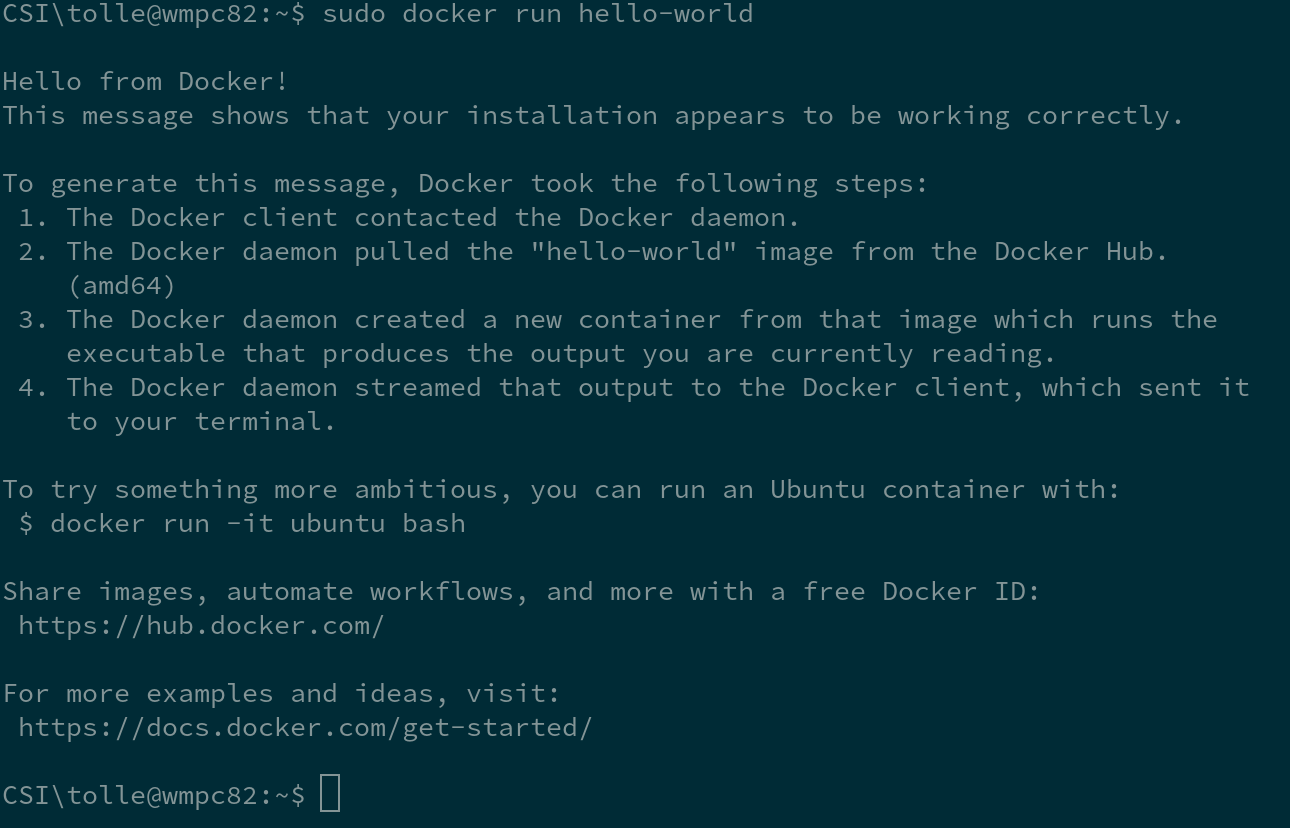
\includegraphics[width=0.5\textwidth]{figures/docker-installation-success.png}
    \end{figure}
\end{frame}


\begin{frame}{(Continuous) Integration of scientific software}
    \framesubtitle{Hands on: setup a Gitlab runner III (install Gitlab runner)}
    Using instructions from \href{https://docs.gitlab.com/runner/install/linux-repository.html}{Gitlab documentation} for Ubuntu:
    \begin{enumerate}
        \item curl -L "https://packages.gitlab.com/install/repositories/runner/gitlab-runner/script.deb.sh" | sudo bash
        \item sudo apt-get install gitlab-runner
    \end{enumerate}
\end{frame}
